% Possible reviewers that I know personally include:
% - Chris Fields
% - Denis Baurain
% - Daisie Huang
% In addition, there are people that appear to be users but that I don't know:
% - Hayward, Alexander 
% - Jern, Patric
% The general idea here is that these are people I haven't published with (yet).
% The BioPerl people's page provides a murderer's row of other candidates, though
% quite a few I already have published with, so there's a potential for COI.
% Here's the list: https://github.com/orgs/bioperl/people
% Also, all people on the previous publication, or people that have since 
% been added to the Acknowledgements in the README.md are obviously out.



\documentclass{bioinfo}
\copyrightyear{2017} \pubyear{2017}

\access{Advance Access Publication Date: Day Month Year}
\appnotes{Applications Note}

% Application Notes (up to 2 pages; this is approx. 1300 words or 1000 words plus one figure)

\begin{document}
\firstpage{1}

\subtitle{Phylogenetics}

\title[short Title]{The Bio::Phylo libraries for phylogenetic data analysis, version 2.0}
\author[Sample \textit{et~al}.]{Rutger A. Vos\,$^{\text{\sfb 1,2}*}$ and Hannes Hettling\,$^{\text{\sfb 1}}$}
\address{$^{\text{\sf 1}}$Naturalis Biodiversity Center, Leiden, P.O. Box 9517, 2300RA, The Netherlands \\
$^{\text{\sf 2}}$Institute of Biology Leiden, Leiden University, Leiden, P.O. Box 9500, 2300RA, The Netherlands}

\corresp{$^\ast$To whom correspondence should be addressed.}

\history{Received on XXXXX; revised on XXXXX; accepted on XXXXX}

\editor{Associate Editor: XXXXXXX}

\abstract{\textbf{Motivation:} Phylogenetic analysis is a broad and expanding field that
requires versatile programming toolkits to manage the various data types, file formats,
and needs for scalability, simulation, visualization, and data exploration.\\
\textbf{Results:} We present version 2.0 of the Bio::Phylo libraries for phylogenetic data
analysis. This new release represents a rewrite of the architecture, allowing for 
extensions that improve speed and persistence, as well as increased functionality in terms 
of analysis, data reading and writing, and visualization.\\
\textbf{Availability:} The package is released as open source software under the same terms as 
Perl itself and available from the comprehensive Perl archive network as well as directly
from the source code repository.\\
\textbf{Contact:} \href{rutger.vos@naturalis.nl}{rutger.vos@naturalis.nl}\\
\textbf{Supplementary information:} Supplementary data are available as \texttt{doi:10.5281/zenodo.1039210}}

\maketitle

% RAV: here are some useful syntax tricks that we will need to observe:
% - refer to figures like so: 'Figure~\ref{fig:01}'
% - citations like this: '\citep{Bag01}' or like that: '\citet{Bag01}', citep is 
%   parenthisized, citet is in-text
% - equations as follows:
% \begin{equation}
% \sum \text{\it x}+ \text{\it y} =\text{\it Z}\label{eq:01}\vspace*{-10pt}
% \end{equation}
% which can then be referenced as Equation~(\ref{eq:01})

\section{Introduction}

Phylogenetic data is multi-faceted, encompassing morphological observations, molecular 
sequences, biological taxa, and tree and network topologies, and is ubiquitous in a 
variety of research fields including comparative genomics, systematics, evolution, 
biodiversity research, and ecology. The types of operations that are performed on 
phylogenetic data range from data cleaning, integration, and conversions, to simulation,
character analysis and inference, and visualization. Flexible programming toolkits that
operate on phylogenetic data and aid in scripting these operations are therefore very 
useful and available in a variety of programming languages. Bio::Phylo \citep{Vos2011} is 
the most versatile toolkit for handling phylogenetic data in the Perl programming
language.

Conceived about ten years ago \citep{Vos2006,Vos2017}, Bio::Phylo has been under
ongoing development ever since. Numerous people have contributed to it, by writing code 
- as volunteers and Google Summer of Code students - by submitting bug reports, and by 
providing inspiration and impetus in larger collaborative networks (e.g. 
\citet{Stoltzfus2010}, \citet{Koureas2016}, \citet{Koureas2016a}) and hackathons (e.g. 
\citet{Lapp2007}, \citet{Katayama2010}, \citet{Katayama2011}, \citet{Katayama2013}, 
\citet{Stoltzfus2013}, \citet{Katayama2014}, \citet{Vos2014}). In the process, additional
requirements surfaced, which have been addressed by a rewrite of the internal architecture
and the addition of functional modules. These have been integrated in a version 2.0
release, which we present here.

\section{Design}

In `object-oriented' programming, the different concepts within the problem domain that
the software addresses are modelled as different classes (e.g. a class to model 
phylogenetic trees, and one to model multiple sequence alignments) that inherit some of 
their functionality from other such classes. For example, a class that represents the 
blueprint for a multiple sequence alignment might inherit certain generalized attributes 
of character state matrices (e.g. the number of characters and taxa) from a `super-class'. 
In turn, this multiple sequence alignment class can be inherited from to create a 
blueprint for a more specialized class, for example one that models amino-acid alignments. 

The object-oriented programming paradigm allows other programmers to extend the 
functionality of toolkits by inheriting from classes to address additional use cases, for 
example by improving performance in various ways. Bio::Phylo has always allowed for this, 
but the version 1.0 design made this relatively cumbersome because a lot of functionality 
would have to be re-implemented for any newly created class to integrate well in the rest 
of the toolkit. In the new design, each class has been reworked into two separate modules, 
one that performs the actual changes to any data associated with the class, and one that 
performs all the other user-friendly operations that do not directly affect the data. With 
this new design, a new class that only re-implements the changes to the data can re-use 
all the other operations, and thus be much more compact and easily written. In addition, 
the integration of such new classes has been made far more flexible (by adopting, in the 
parlance of software design patterns \citep{Gamma1995}, the `Factory' pattern throughout).

The usefulness of this change of design is demonstrated by two optional extension packages
that can be installed alongside Bio::Phylo. One of them, Bio::PhyloXS, serves as a drop-in
replacement of the core data objects in Bio::Phylo, re-implemented in the C programming
language. Because C is a very fast, compiled language, having some of the core 
functionality (e.g. setting and fetching data properties) leads to significant speed 
increases: a simple benchmark test where a small tree topology is constructed and then
traversed executes about 700\% faster using this extension. (Note, however, that bindings
between C and Perl are fraught with challenges due to the complexity of the Perl API and
the differences in memory management on different architectures. Hence, this application
should currently be considered 'experimental'.) The second optional extension,
Bio::Phylo::Forest::DBTree, allows very large trees to be stored into, and accessed from,
a simple SQLite database. This means that these trees never have to be loaded in working
memory, and that, once stored in the database, there is no "file reading" step. The 
typical application for this is to store static, immutable trees. To demonstrate this, we
make available database files that were created by indexing the releases listed in 
Table~\ref{table1}.

\begin{table}[!t]
\processtable{Large, published phylogenies made available as database files\label{table1}} 
{\begin{tabular}{@{}ll@{}}\toprule \textbf{Project} & \textbf{Database files}\\\midrule
PhyloTree \citep{Oven2009}         & {\small 10.6084/m9.figshare.4620757.v1} \\
D-Place \citep{Kirby2016}          & {\small 10.6084/m9.figshare.4620217.v1} \\
NCBI taxonomy \citep{Federhen2011} & {\small 10.6084/m9.figshare.4620733.v1} \\
Greengenes \citep{Desantis2006}    & {\small 10.6084/m9.figshare.4620214.v1} \\\botrule
\end{tabular}}{}
\end{table}


\section{Data input and output}

In addition to the file formats already supported in previous releases of Bio::Phylo, 
several new formats are now read and/or written. Specifically, PhyloXML \citep{Han2009},
New Hampshire eXtended (NHX, \citet{Zmasek2001}), the extensions added to the NEXUS
standard by the programs TreeAnnotator and Figtree \citep{Rambaut2007}, and a `badgerfish'
mapping of NeXML \citep{Vos2012} to JSON can now both be read and written. In addition, 
several response formats from web services (namely, the DarwinCore archive format returned 
by GBIF \citep{Baker2014}, the response format from the TaxoSaurus.org service 
\citep{Stoltzfus2013}, and the response documents of uBio.org) as well as FASTQ 
\citep{Cock2009} files can be read. Data files for Hennig86 \citep{Farris1988} and for
the haplotype `Network' program (fluxus-engineering.com) can be written. 

Support for RDF is experimental: RDF/XML triples can be written by way of a two-step 
process that first exports data as NeXML and then transforms this to statements that 
obtain terms from CDAO \citep{Prosdocimi2009}; this is the same approach and uses the 
same transformation stylesheet as TreeBASE \citep{Piel2009}). RDF graphs can also be 
`read' in the sense that a graph can be loaded and interrogated with SPARQL queries to 
extract statements that map onto Bio::Phylo's object model. At present, this means that 
annotated taxa and tree topologies can be extracted from CDAO/RDF, but character data 
cannot.

\begin{figure}
\centerline{\includegraphics{tree_detail_cropped.eps}}
\caption{Mammal supertree \citep{Bininda2007} decorated with log-transformed body 
mass \citep{Jones2009} as branch colors and monophyletic genera as labeled braces; detail 
and full tree (inset). Image produced as per the workflow described on 
http://rvosa.github.io/bio-phylo/doc/examples/integration/}
\label{figure1}
\end{figure}

\section{Analysis, modification, and simulation}

From its first versions onwards, Bio::Phylo has implemented numerous algorithms for 
computing topological indices, simulating new topologies, and adjusting them 
algorithmically. Some of the simulation methods were developed and discussed by 
\citet{Hartmann2010}, while some of the topology index algorithms were explored by
\citet{Martyn2012}. To the existing topology indices, some additional methods were added: 
the Euclidean distance between trees (see \citet{Kuhner1994}) and the number of `cherries'
in a given topology (see \citet{McKenzie2000}) can now be computed. To the algorithms
that adjust topologies have been added methods to obtain ultrametric trees using the mean 
path lengths method of \citet{Britton2002}, by making node ages proportional to clade size 
(as per \citet{Grafen1989}), and using an implementation of Stadler's algorithm for 
computing the relative order of speciation or coalescence events on a given phylogeny 
\citep{Gernhard2006}.

By implementing a bridge between Bio::Phylo's library code and the R programming language,
additional functionality has become accessible. So far, this has been wrapped in methods
to estimate the parameters of the birth/death process and use these to simulate replicates
of the input tree (using `ape', \citet{Paradis2004}); and methods to estimate the 
parameters of state transition models for binary characters and DNA sequences (using
`phangorn', \cite{Schliep2010}; `phylosim', \citet{Sipos2011}; and `phytools', 
\citet{Revell2012}). To encapsulate these state transition models, a class hierarchy has
been implemented that represents some of the common substitution models (i.e. JC69,
HKY85, GTR, F81, K80) such that they can be serialized to the syntax of commonly used 
programs for phylogenetic inference. In addition, this facility to select substitution 
models has been combined with a (tree-based) sequence simulator to allow multiple sequence 
alignments to be replicated.

\section{Visualization}

The ability to visualize phylogenies as rooted, rectangular cladograms and phylograms in
vector formats (SVG being best supported) has always existed in Bio::Phylo. This included
functionality to paint branches, add pie charts to nodes, collapse clades as triangles,
and influence styling (such as branch thickness; fonts and their size, weight, and style).
To this has been added in v2.0.0 the ability to draw unrooted and radial tree projections,
and the option to mark up higher taxa in labeled braces (straight or arched, depending on 
projection). Figure~\ref{figure1} demonstrates some of this new functionality.

\section{Impact and re-use}

As of time of writing (October 2017), the first version of Bio::Phylo has been cited 35
times. Among these, the papers with the highest impact used Bio::Phylo in analyses in
phylogenomics and comparative genomics (e.g. see \citet{Roure2012,Hayward2013,Smet2013}).

Several infrastructural projects depend on Bio::Phylo. These include the BioPerl project 
\citep{Stajich2002}, which uses it for reading and writing NeXML. This usage is promoted
by the interface compatibility between the two projects: the core data objects of 
Bio::Phylo, i.e. trees, tree nodes, sequence alignments, and so on, can be used directly
in BioPerl. Also, the TreeBASE project \citep{Piel2009} uses Bio::Phylo for certain
server-side maintenance tasks, and the SUPERSMART project \citep{Antonelli2017}, as well
as the BioVeL services that expose it \citep{Hardisty2016}, are deeply integrated with 
Bio::Phylo (and drove some of the development of new functionality). 

In addition, several single-purpose programs and pipelines use Bio::Phylo. These include
the Monophylizer web service for assessing monophyly in gene trees 
\citep{Mutanen2016,Mutanen2016a}; the CopyRighter tool for improving the accuracy of 
microbial community profiles through lineage-specific gene copy number correction
\citep{Angly2014}; and the PhyloMatch pipeline to discover highly phylogenetically 
informative genes in sequenced genomes \citep{Ramazzotti2012}.

\section{Availability}

All revisions of the source code are available from the source code repository at
http://github.com/rvosa/bio-phylo. The latest stable release version, which over time may
fall behind the latest source code revision, is available from the Comprehensive Perl 
Archive Network (CPAN) at http://search.cpan.org/dist/Bio-Phylo. Accompanying this 
publication is a uniquely identifiable release, stamped with a Digital Object Identifier 
(DOI) issued by Zenodo.org: \texttt{doi:10.5281/zenodo.1039210}.

As is a common convention in Perl software releases, a dual licensing scheme applies to
Bio::Phylo - both the Artistic License 
(https://github.com/rvosa/bio-phylo/blob/master/COPYING) as well as the GNU General Public 
License (https://github.com/rvosa/bio-phylo/blob/master/LICENSE) applies. This is 
generally interpreted to mean that you are free to choose whichever of these licenses fits 
best with your own project, should you want to reuse all (or part) of Bio::Phylo. This is 
certainly the spirit: feel free to use these libraries however you see fit. No warranties.

\section*{Acknowledgements}

The following people have contributed code to the project: Florent Angly, Jason Caravas, 
Klaas Hartmann, Mark A. Jensen, Moritz Lenz, Chase Miller, Aki Mimoto, and Jan Willem 
Wijnands. The following people have provided feedback through bug reports and reviews:
Denis Baurain, Chris Fields, Shlomi Fish, Jean-Marc Frigerio, Andreas J. K\"{o}nig, Hilmar 
Lapp, Nicolas Lenfant, S\'{e}bastien Moretti, Slaven Rezi\'{c}, \texttt{Seiler}, and
\texttt{scorpio17}. Mannis van Oven has been very helpful in providing the data dumps of
the PhyloTree.org project that were indexed as database files (in Table 1). The principal
investigators of the labs in which RAV has done his research have all allowed and 
encouraged the development of Bio::Phylo. These are Arne Mooers, Wayne Maddison, and Mark
Pagel, and now Naturalis Biodiversity Center. We are grateful to all these people for 
their support.

\section*{Funding}

The research leading to these results has received funding from the European Community's 
Seventh Framework Programme (FP7/2007-2013) under grant agreement no. 237046.

\bibliographystyle{natbib}

\bibliography{document}

\end{document}
